% !TEX encoding = UTF-8
% !TEX TS-program = pdflatex
% !TEX root = ../thesis.tex

%**************************************************************
\chapter{STATO DELL'ARTE}
\label{Capitolo2}
\thispagestyle{empty}

Il tema della guida autonoma si sta sempre più affermando come importante 
oggetto di studio nella comunità scientifica. Visto il grande impiego di sistemi 
basati sul Machine Learning, in particolare le reti neurali, in questa sezione 
verranno introdotti alcuni concetti atti a rappresentare sia la struttura di tali 
sistemi che la loro influenza nell’ambiente automotive. 

\section{Reti Neurali Biologiche}
Il cervello umano ha la capacità di sfruttare la sua struttura di neuroni in modo 
da eseguire più calcoli rispetto a un comune computer. Mediamente ogni cervello 
contiene un numero di neuroni pari a $10^{11}$. La struttura di un neurone biologico 
è quello mostrata in figura (\ref{biological neuron}):
\begin{figure}[H]
    \centering
    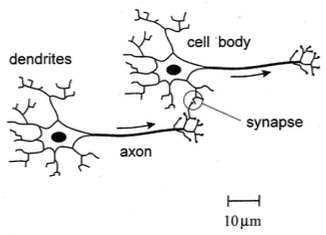
\includegraphics[width = 0.6 \linewidth]{images/biological neuron.png}
    \centering
    \caption{Composizione di due neuroni biologici.}
    \label{biological neuron}
\end{figure}
Da come possiamo notare, esistono vari componenti che costituiscono un 
neurone. In particolare, abbiamo i \emph{dendriti} che rappresentano gli ingressi di un 
neurone mentre le uscite sono rappresentare dagli \emph{assoni}. Su ogni assone viaggia 
un impulso elettrico generato dal neurone stesso quando questo si trova in uno 
stato attivo. Ogni neurone è connesso a migliaia di suoi simili ed ogni 
comunicazione fra questi avviene mediante le sinapsi. Quando l’impulso raggiunge 
proprio le sinapsi, questo provoca il rilascio di sostanze chimiche che attraversano 
la giunzioni ed entrano all’interno di altri neuroni. Ci sono due tipologie di sinapsi, 
eccitatori e inibitori. La prima tipologia permette di aumentare la probabilità che 
un neurone si attivi. Tale probabilità è determinata dal peso associato ad ogni 
sinapsi. Avendo multipli collegamenti, ogni neurone effettua una specie di somma 
pesata degli ingressi che, se maggiore di una determinata soglia, può provocare la 
sua attivazione. 

\section{Reti Neurali Artificiali}
Una rete neurale artificiale è un modello computazionale che, a partire da dei dati 
di input, riesce a produrre un output mediante un meccanismo ispirato a quello 
del cervello umano. Alla base di questa similitudine, tali reti prendono il nome di 
\emph{Artificial Neural Networks (ANN)}. Le prime reti neurali, nate attorno gli anni 
’50, basavano il loro funzionamento sui cosiddetti \emph{percettroni}, neuroni artificiali in 
grado di apprendere e di accumulare esperienza. Ogni rete neurale è composta da 
strati di neuroni, comunemente chiamati \emph{layers}. I dati di input saranno processati 
dai neuroni presenti nell’input layer e da qui, i risultati ottenuti, si propagheranno 
verso i layer nascosti (hidden layers) fino a raggiungere il layer finale di output (Fig. \ref{network structure}).
\begin{figure}[H]
    \centering
    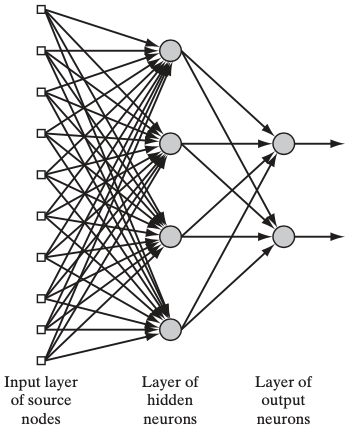
\includegraphics[width = 0.6 \linewidth]{images/netwrok structure.png}
    \centering
    \caption{Struttura di una rete neurale a più livelli.}
    \label{network structure}
\end{figure}
Grazie a questa massiccia interconnessione, le reti neurali artificiali sono in 
grado non solo di imitare il comportamento del cervello umano ma anche di 
svolgere diversi compiti grazie a una opportuna fase di apprendimento. 

\section{Algoritmi di apprendimento}
Lo scambio di dati tra i vari neuroni consente alla rete neurale di poter generalizzare 
anche con dati mai visti nel training set. Questo processo prende il 
nome di “\emph{Apprendimento}”. Una rete neurale artificiale può avere vari tipi di 
apprendimento: \emph{Supervisionato, Semi-Supervisionato, Non-Supervisionato} e con \emph{Rinforzo}. La scelta 
di quale usare dipende dalla tipologia della rete e dal suo campo di applicazione

\subsection{Apprendimento Supervisionato}
In questa tipologia di apprendimento, l’input fornito alla rete contiene una serie di 
dati etichettati. L’apprendimento supervisionato è solitamente utilizzato sia nel 
conteso della classificazione, dove  si vuole mappare le etichette di input a quelle 
di output, che nel contesto della regressione, dove si mira a mappare l’input a un 
output continuo. La corretta associazione comporta una buona generalizzazione 
da parte del modello. L’apprendimento migliora grazie ad una continua variazione 
dei pesi. Questo tipo di apprendimento è svolto utilizzando una ben nota tecnica 
presente allo stato dell’arte, chiamata \emph{Back-Propagation}. La complessità di questo 
tipo di apprendimento deriva dalla quantità di dati presenti nel training set. 
Affinché la rete riesca a generalizzare al meglio, il training set dev’essere composto 
da un numero di esempi adeguato. La giusta quantità di esempi è utile a prevenire 
spiacevoli situazioni di underfitting o di overfitting della rete.

\subsection{Apprendimento Non-Supervisionato}
Quando una rete neurale è sottoposta ad un simile apprendimento, questa riceve 
in input dei dati privi di etichettatura o non strutturati. Lo scopo della rete, 
o del modello, è quello di estrarne una rappresentazione e creare dei cluster 
rappresentativi. Ci sono delle tecniche a supporto di questa tipologia di apprendimento, 
una fra queste è la riduzione della dimensionalità che è applicata in fase 
di pre-elaborazione delle features avente l’obiettivo di eliminare il rumore dai dati 
quando questi sono presenti in grandi quantità. 

\subsection{Apprendimento Semi-Supervisionato}
Un set di input composto da dati etichettati e non, costituisce un sistema di apprendimento 
semi-supervisionato. Questa tipologia di apprendimento rappresenta 
un sistema che si interpone tra i due precedentemente spiegati. I modelli che fanno 
uso di questo approccio di solito utilizzano una piccola quantità di dati etichettati 
e una grande quantità di dati non etichettati. Tale apprendimento porta alla 
creazione di un modello più flessibile rispetto a quello ottenuto dall’apprendimento 
supervisionato.

\subsection{Apprendimento con Rinforzo}
L’ultimo tipo di apprendimento automatico è chiamato Apprendimento con 
Rinforzo. Il suo scopo è quello di costruire un sistema, comunemente chiamato 
\emph{agente}, che abbia l’obiettivo di migliorare le sue performance interagendo con 
l’ambiente che lo circonda. Il miglioramento dell’intero sistema avviene mediante 
dei feedback chiamati appunto rinforzi. Quest’ultimi non hanno nulla a che fare 
con etichette o valori di verità, ma rappresentano un livello di qualità delle azioni 
intraprese dal sistema. Pertanto, differentemente da un sistema supervisionato, 
non ci sono mappature tra l’input e l’output.

\section{Tipologie di reti neurali}
Esistono diverse tipologie di reti neurali, tra queste abbiamo:
\begin{itemize}
    \item \emph{Reti neurali feed forward (FNN)}
    \item \emph{Reti neurali ricorrenti (RNN)}
    \item \emph{Reti profonde (DNN)}
    \item \emph{Reti convoluzionali (CNN)}
\end{itemize}
Nel seguente elaborato verranno trattate solamente le reti neurali convoluzionali 
ma, prima di introdurle, al fine di capire il loro funzionamento, è necessario 
introdurre prima le reti neurali feed-forward, dette anche reti neurali a catena 
aperta.

\subsection{Reti neurali Feed-Forward}
Per facilitare la comprensione del funzionamento di una comune rete neurale, 
si potrebbe partire dallo studio del comportamento di una feed-forward neural 
network. Questa tipologia di rete può essere vista come una funzione matematica 
non lineare capace di trasformare dei dati di input $x=(x_1, \dots, x_m)$, in dati in 
output $y=(y_{k1}, \dots, y_{kn})$. Quello che accade è quindi una transizione delle variabili 
indipendenti ($X_k$) in variabili dipendenti($Y_k$). Un altro componente importante, 
facente parte della funzione, è costituita da un insieme di valori $w=(w_{k1}, \dots, w_{km})$ 
chiamati pesi. Ogni peso è rappresentato da un numero reale che riflette il grado 
di importanza di una data connessione, tra due neuroni, in una rete neurale \cite{02}. I 
pesi possono subire dei cambiamenti in base alla tipologia di apprendimento della 
rete. Una buona configurazione dei pesi riduce l’errore di predizione e pertanto 
migliora l’output del modello. Possiamo quindi considerare la rete come una 
funzione nella forma $y = y(x;w)$, dove $y$ sta a rappresentare una funzione di $x$ 
e che a sua volta è parametrizzata da $w$. Riprendendo il discorso dei neuroni, 
McCulloch e Pitts  \cite{Chakraverty2019} definirono un modello matematico in grado di rappresentarli.
In particolare, il compito di ogni singolo neurone è rappresentato nella figura (\ref{neural neuron}).
\begin{figure}[H]
    \centering
    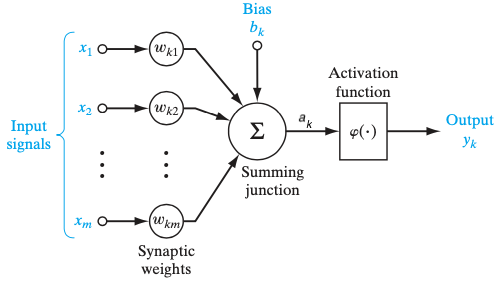
\includegraphics[width = \linewidth]{artificial neuron.png}
    \centering
    \caption{Neurone artificiale.}
    \label{neural neuron}
\end{figure}
Da come possiamo notare, un neurone è una semplice funzione non lineare che 
riceve in input una serie di input $X_{kn}$ e produce in output una variabile $y_k$. Il 
calcolo dell’output, di ogni singolo neurone, è composto da una sommatoria degli 
input, di segno positivo o negativo, moltiplicati prima con i corrispettivi pesi 
e successivamente sommati con una variabile, chiamata bias (pregiudizio), che 
corrisponde alla soglia di attivazione del neurone.
\begin{equation}\label{artificial}
    a_k = \sum_{j=0}^m w_{kj}x_j + b_k 
\end{equation}
Una soglia è utile per determinare se l’informazione in ingresso “$x$” debba essere 
elaborata oppure scartata. Di solito vi è sempre un input $X_0=1$ che renderebbe 
il bias $ b_k $ uguale uguale al primo peso $W_0$, pertanto la formula (\ref{artificial}) può anche 
essere scritta come:
\begin{equation}\label{artificial without bias}
    a_k = \sum_{j=0}^m w_{kj}x_j
\end{equation}
Per poter determinare il valore $y$, dopo aver ottenuto “$a$”, si utilizza una “\emph{funzione di 
attivazione}” non lineare $\varphi(\cdot)$:
\begin{equation}\label{activation function}
    y_k = \varphi(a) = \varphi(\sum_{i=0}^k w_ix_i)
\end{equation}
L’uscita $y$ determinerà l’attivazione del prossimo neurone. Se il valore ricevuto è 
maggiore di zero, allora il neurone si attiverà, altrimenti resterà spento.
\begin{equation}\label{activation function}
    y_k = \left\{
        \begin{array}{rl}
        1 & \mbox{if } a_k \geq 0 \\
        0 & \mbox{if } a_k < 0
        \end{array}
        \right.
\end{equation}
Esistono varie funzioni di attivazione, diverse sono elencate in figura (\ref{activation function}).
\begin{figure}[H]
    \centering
    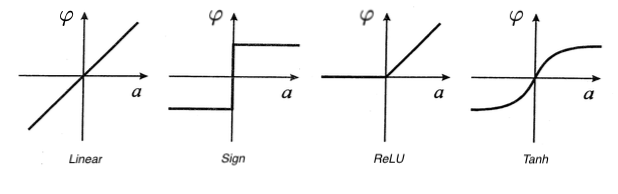
\includegraphics[width = \linewidth]{activation functions.png}
    \centering
    \caption{Varie funzioni di attivazione.}
    \label{activation functions}
\end{figure}